\chapter{Implémentation de la blockchain}
\label{ch:realisation}

\section{Introduction}

Dans ce chapitre est présenté l'implémentation de la blockchain. Il explique les choix d'implémentation et montre comment la blockchain fonctionne. L'implémentation actuelle de la blockchain se limite à une utilisation locale hors-ligne. Comme pour la partie proof of space, la blockchain est implémentée en Rust et certaines parties du code source seront présentées.

Le code sources est un workspace cargo contenant plusieurs crates. Une crate est un projet Rust. Le but est de diviser le code pour mieux régner.

Les crates importantes sont les suivantes :

\begin{itemize}
  \item \textbf{crypto}: traits et structures liés à la cryptographie
  \item \textbf{ledger}: crate gérant le registre, les blocs et les transactions
  \item \textbf{merkletree}: algorithme pour l'arbre de Merkle
  \item \textbf{node}: client en ligne de commandes
  \item \textbf{pospace}: implémentation du proof of space
  \item \textbf{storage}: crate gérant le stockage des informations
\end{itemize}

\section{Cryptographie}

La cryptographie est au cœur d'une cryptomonnaie, le choix des primitives est donc très important. Une crate est dédiée entièrement aux primitives cryptographiques utilisée afin de les regrouper plus simplement.

Le 1er choix est concernant les signatures. Il existe plusieurs algorithmes pour faire des signatures mais celui choisi pour ce projet est \textbf{EdDSA}, plus précisément \textbf{Ed25519}. C'est un algorithme de signature basé sur les courbes elliptiques sûr et éprouvé et qui a l'avantage de générer des clés plus petites que RSA donc pratique pour une blockchain. De plus il existe une librairie en Rust appelée \emph{ed25519-dalek} qui est populaire. C'est celle qui sera utilisée pour ce projet.

Pour l'intégration au projet de la librairie, des traits sont utilisés pour encapsuler le fonctionnement et permettre une migration facilitée en cas de changement de librairie.

Un deuxième point concernant le crypto est les fonctions de hachages. Dans l'algorithme de proof of space, c'est \textbf{BLAKE3} qui a été utilisé pour des raisons de performance. C'est pourquoi c'est aussi BLAKE3 qui est utilisé pour la blockchain sauf pour les signatures où c'est du SHA-512 (requis par la librairie ed25519-dalek). En plus, la librairie Rust de BLAKE3 est maintenue par les créateurs de BLAKE3 donnant tout de suite plus de crédibilité à la cette dernière.

\section{Transactions}

L'objectif est de réaliser un système de paiement décentralisé. Les transactions sont alors un élément nécessaire à la blockchain. Ces signatures doivent pouvoir être signées, ce qui sera expliqué dans la section \ref{sec:signature}. Pour simplifier par rapport à d'autres blockchains existantes, les transactions contiendront juste un timestamp, une adresse de destination, le montant de la transaction, des frais de transaction et une signature. Le tout en différentes structures Rust :

\inputsourcecode{rust}{"sources/transaction_1.txt"}{Structure d'une transaction}

L'idée dernière cette séparation entre signature et payload est que c'est la payload de la transaction qui sera signée. C'est donc tous les éléments de la \verb|TransactionPayload| qui seront hachés et signés et placé dans une \verb|TransactionSignature|.

\inputsourcecode{rust}{"sources/transaction_2.txt"}{Structure d'une signature de transaction}

On peut voir que le code des transactions est générique sur les types de signatures et de clés publiques. Cela permet d'utiliser ces structures avec d'autres moyens de signature que Ed25519 si besoin dans le futur.

\inputsourcecode{rust}{"sources/transaction_3.txt"}{Structure des éléments d'une transaction}

Le timestamp est ici une simple indication et en aucun cas un moyen sécurisé de vérifier qu'une transaction a eu lieu avant un autre. Ceci car l'émetteur de la transaction peut tout simplement choisir la date et il est difficile de vérifier si c'est la vérité.

\section{Adresses}

Les \emph{adresses} sont un moyen d'identifier un compte sur la blockchain. Elle est dérivée de la clé publique ce qui veut dire qu'on peut passer d'une $pk$ à une adresse mais pas inversement. Une \emph{adresse} est un tableau de 22 octets. Pourquoi 22 octets au lieu de 32 octets, la taille d'une clé publique ? Parce que cela rend une chaîne de caractère plus petite et plus facilement utilisable. L'adresse est composé de 2 octets pour la version, 16 octets provenant de l'adresse et 4 octets pour la checksum. 16 octets permet d'avoir $2^{16 \times 8}$ adresses différentes ce qui est amplement suffisant pour une utilisation dans le futur. La checksum permet d'éviter les erreurs de frappe si on saisi une adresse à la main par exemple. Elle représente les 4 premiers octets du hash de la payload.

\inputsourcecode{rust}{"sources/address.txt"}{Création d'une adresse à partir d'une clé publique}

Pour l'affichage, c'est l'encodage \emph{base58} qui est utilisé comme pour le Bitcoin. Cela permet d'éviter les confusions avec des charactères qui se ressemblent comme l (L minuscule) et I (i majuscule), 0 (zéro) et O (lettre o) par exemple.

\section{Merkle tree}

L'arbre de Merkle est un arbre binaire de hash. Un arbre dans lequel chaque nœud est concaténé avec son frère et haché pour obtenir le nœud parent et ainsi de suite jusqu'à obtenir le nœud racine. Cette structure est très pratique car elle permet de savoir efficacement si un nœud appartient à l'arbre sans avoir tous les nœuds à disposition, seulement $\log_2(N)$ hashs, $N$ étant le nombre d'éléments à hacher au départ.

Cette structure est notamment utilisée pour hacher les transactions au sein d'un bloc. On stocke dans le bloc la racine de l'arbre de Merkle. Comme cela, si un utilisateur veut savoir si une transaction appartient à un bloc, il n'a pas besoin de télécharger toutes les transactions du bloc, seulement le hash du frère, de l'oncle, grand-oncle etc... jusqu'à la racine ce qui donne pour un bloc de 1000 transactions seulement $\log_2(1000) \approx 10$ hashs.

Une implémentation simple a été réalisée pour ce projet sans librairie. Cependant elle ne permet pas encore de vérifier une transaction de manière optimale comme présenté ci-dessus. Cela fait partie d'une amélioration possible pour le projet.

\section{Signatures}
\label{sec:signature}

Pour être valide, une transaction doit être signée par l'utilisateur qui souhaite envoyer de l'argent. Pour ce faire, on signe la payload de la transaction. Il y a donc une méthode implémentée pour la structure \verb|TransactionPayload| qui permet de signer ses éléments et de retourner une \verb|Transaction|.

\inputsourcecode{rust}{"sources/signature_1.txt"}{Signature d'une transaction}

On peut remarquer qu'un \verb|CONTEXT| est utilisé à la ligne 3. C'est pour rendre unique une signature par rapport à un context donné car les signatures EdDSA sont déterministes. C'est-à-dire que pour une même clé privée et un même message, l'algorithme donnera la même signature à chaque fois à la différence de ECDSA par exemple où la signature sera différente. Ce contexte permet d'avoir une séparation pour différentes utilisations.

\section{Blocs}

Maintenant que les transactions sont signées, il faut les assembler au sein d'un \emph{bloc}. Le bloc est représenté sous la forme suivante :

\inputsourcecode{rust}{"sources/bloc_1.txt"}{Structure d'un bloc}

Il possède une hauteur qui indique où est-ce qu'il se situe dans le chaîne, un timestamp indiquant quand le bloc a été créé, utile car modifiable facilement si aucune preuve n'est trouvée pour le hash du bloc; un hash, le hash du bloc précédent ($\mathsf{hauteur} - 1$), la liste des transactions, la racine de l'arbre de Merkle et une preuve.

Certains types sont optionnels car le premier bloc, le \emph{genesis} n'as pas besoin de toutes les données comme le hash du bloc précédent par exemple.

Pour vérifier un bloc, on vérifie d'abord son hash puis on vérifie les transactions à l'intérieur. La validation des transactions concerne la vérification de la signature. Les autres vérifications comme le solde d'une adresse se font au niveau du registre car au niveau d'un bloc on a aucune notion de solde encore.

Le registre, c'est la blockchain. Il regroupe tous les blocs ensemble et permet de vérifier ainsi l'ensemble des transactions. On peut ajouter un bloc au registre à partir de transactions existantes, par exemple des transactions reçues à partir du réseau. Ce dernier va alors créer un nouveau bloc à la suite de la chaîne.

Le registre permet également de récupérer le solde d'une adresse.

La sérialisation et le stockage de la blockchain se font bloc par bloc à l'aide de la librairie Borsh.

\section{Tests}

Comme pour le proof of space, l'entièreté du projet est testé avec des tests unitaires afin de vérifier le bon fonctionnent du registre, blocs, transactions et autres. Notamment pour tester les cas limites dans certaines situations ou bien des erreurs particulières.

L'ensemble du projet gère les erreurs de manière ciblée avec les librairies \emph{thiserror} et \emph{anyhow} permettant de créer des erreurs personnalisées et de les gérer de manière intuitive. C'est-à-dire que la majeur partie des fonctions retournent un \verb|Result|, ce résultat sera traité dans la fonction << main >> et grâce à anyhow, des contextes peuvent être ajoutés pour donner plus d'indications sur une erreur.

Afin de pouvoir tester la blockchain avec le protocole de proof of space, une interface en ligne de commande a été réalisée. Il est possible de l'essayer avec Cargo, l'utilitaire pour manager les projets Rust. Il faut tout d'abord récupérer le code source disponible sur GitHub: \url{https://github.com/spaceframeos/spaceframe}. Ensuite on peut lancer la commande suivante :

\begin{shellcmd}
  cargo run --release --bin spaceframe-node -- init -k 17
\end{shellcmd}

Cela va initialiser le plot pour pouvoir trouver des preuves par la suite. La valeur de $k$ est au choix mais 17 est une bonne valeur pour tester rapidement. On peut ensuite lancer la commande de démonstration pour jouer avec la blockchain :

\begin{shellcmd}
  cargo run --release --bin spaceframe-node -- demo -k 17
\end{shellcmd}

On tombe alors sur une liste d'actions. On peut ajouter une paire de clés (un compte), on peut ajouter un nouveau en bloc, on peut voir les soldes des comptes et voir les blocs présents dans la chaîne.

\begin{figure}[H]
  \centering
  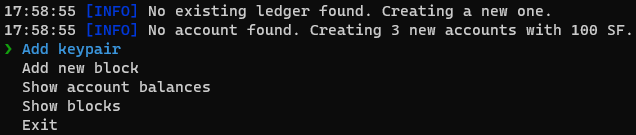
\includegraphics[width=\textwidth]{images/chain_home.png}
  \caption{Liste des actions}
\end{figure}

\newpage

On peut choisir d'ajouter un nouveau bloc en créant d'abord 0, 1 ou plusieurs transactions (c'est possible de créer un bloc sans transaction). Il faut sélectionner la personne qui envoie, celle qui reçoit et le montant.

\begin{figure}[H]
  \centering
  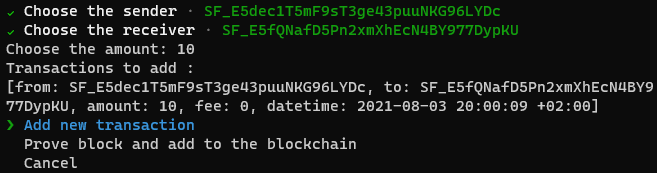
\includegraphics[width=\textwidth]{images/chain_add_transaction.png}
  \caption{Ajout d'une transaction}
\end{figure}

On peut ensuite prouver ce nouveau bloc et l'ajouter à la chaîne. Il est alors possible de consulter les changements au niveau des comptes.

\begin{figure}[H]
  \centering
  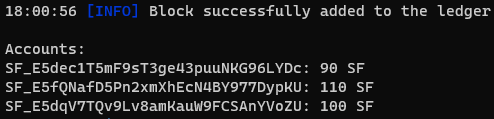
\includegraphics[width=\textwidth]{images/chain_balances.png}
  \caption{Soldes des comptes}
\end{figure}

Le montant a bien été transféré. Maintenant on peut tester d'envoyer 100 avec le 1er compte qui n'a que 90.

\newpage

\begin{figure}[H]
  \centering
  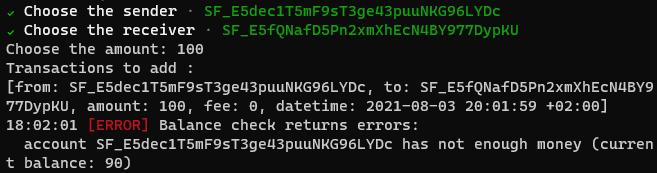
\includegraphics[width=\textwidth]{images/chain_balance_error.png}
  \caption{Erreur de création d'un bloc}
\end{figure}

Au moment de la vérification du bloc, ce dernier est refusé car il contient des transactions dont le signataire n'a pas assez d'argent.

Après cela, il est possible de visualiser les blocs de la chaîne et de les vérifier par la même occasion.

\begin{figure}[H]
  \centering
  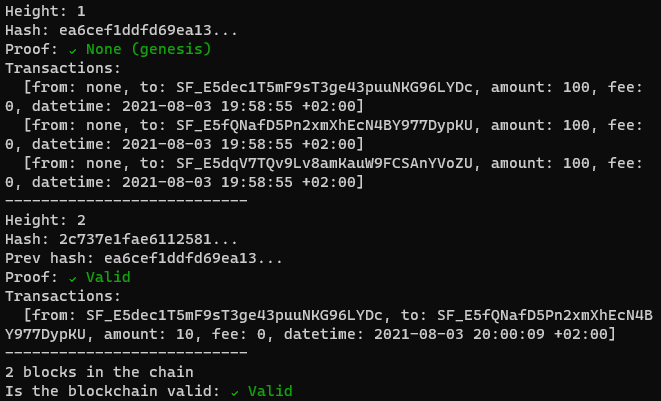
\includegraphics[width=\textwidth]{images/chain_blocks.png}
  \caption{Visualisation et validation des blocs}
\end{figure}

\newpage

On peut également ajouter de nouveaux comptes pour tester grâce à l'action << Add keypair >>.

\begin{figure}[H]
  \centering
  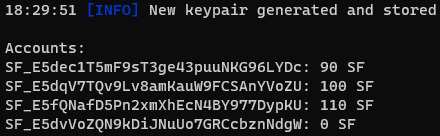
\includegraphics[width=\textwidth]{images/chain_add_keypair.png}
  \caption{Ajout d'un compte de test supplémentaire}
\end{figure}

Ceux-ci auront alors un solde de 0 initialement.